\documentclass[a4paper]{article}
\usepackage[utf8]{inputenc}
\usepackage{amsmath}
\usepackage{amssymb}
\usepackage{mathtools}
\usepackage{amsfonts}
\usepackage{lastpage}
\usepackage{pdfpages}
\usepackage{fancyvrb}
\usepackage[table]{colortbl}
\usepackage{fancyhdr}
\usepackage[linesnumbered, ruled]{algorithm2e}
\usepackage{graphicx}
\SetKwRepeat{Do}{do}{while}%
\usepackage[margin=2.5 cm]{geometry}


\pagestyle{fancy}
\cfoot{Page \thepage\ of \pageref{LastPage}}
\DeclareGraphicsExtensions{.pdf,.png,.jpg}
\author{Sigurdur Oli Arnason (5961181) \\ Victor Petren Bach Hansen (5990025)}
\title{Algorithms \& Networks \\ Exercise 5}
\lhead{Algorithms \& Networks}
\rhead{Exercise 5}

\begin{document}
\maketitle
\section{Independent set and non-standard measures}
\subsection*{i)}
If all vertices have degree 2 then the graph is a disjoint cycle cover of the vertices and we have at most $n/3$ cycles.\\
Find the cycles by choosing a random vertex and recursively adding the vertices you can travel to to the cycle. Remove those vertices from the graph. Repeat until no vertex in graph.\\
For each cycle there are two possible maximum independent sets.\\
\indent Choose some vertex v in the cycle and add it to the set. Then traverse the cycle and add every other vertex until you reach v's neighbor.\\
\indent Choose either of v's neighbors and do the same for that vertex as we did for v.\\
\indent Choose the set that is larger.\\
Do this for all cycles and the maximum independent set is the union of these sets.
\subsection*{ii)}
\subsection*{iii)}
Making $G^1$ removes x with $d(x)=3$ and $w(x)=1$. X has 3 neighbors with degree 2 or 3 but all their degrees go down by one when x is removed so their weights go either from 1 to $1/2$ or from $1/2$ to 0. So the total weight loss is $1+3\cdot 1/2=5/2$
\subsection*{iv)}
We always remove at least as much as in $iii)$
\subsection*{v)}
First note that
\[
c^{5/2}-2=0 \iff c=2^{2/5}
\]
Removing vertices of degree 0 or 1 is done in total in linear time since it always reduces the problem by at least one vertex and never splits it. When working on vertices with degree 3 we create a recursion tree where the problem is always split into two sub-problems where the weight of each sub-problem is at least $5/2$ less than the weight of the current one. If the weight of the tree is less than one then there is no vertex of degree 3 so all vertices are of degree 2 so we can solve in polynomial time. This means that the recursion tree is a binary tree of depth at most $\frac{m(v)}{5/2}$ so the number of leaves is:
\[
2^{\frac{m(v)}{5/2}}=2^{2/5^{m(v)}}=O(2^{2/5^n})=O(c^n)
\]
\subsection*{vi)}
\subsection*{vii)}
\subsection*{viii)}

\section{}
\section{A simple question on Graph Isomorphism}

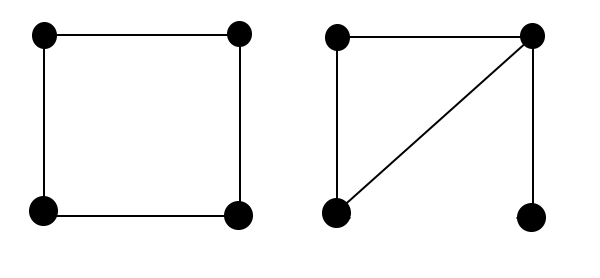
\includegraphics[width=\textwidth]{3}

\section{Number of automorphisms for (uncolored) cycles}
We have n rotations and n reflections so we have $2n$ automorphisms in total.
\section{Isomorphism testing for colored cycles}
\subsection*{i)}
Define a random vertex $v_0$ in cycle $G_1$ as the starting vertex in the cycle  and similarly $u_0$ in cycle $G_2$. Say that $c(v)$ is the color of vertex $v$.\\
For each of the $2n$ color-insensitive automorphisms of $G_1$:\\
Check if $c(w_0)=c(u_0)$ where $w_0$ is the vertex that is mapped to $v_0$ in the automorphism\\
Move to the right in both cycles and check if both vertices have the same color.\\
Repeat until back to $w_0$.\\
If all colors are the same then return YES.
If fails for all automorphisms then return NO.
Each cycle is $O(n)$ and we go $2n$ cycles so the algorithm is $O(n^2)$.
\subsection*{ii)}
Take all color-insensitive automorphisms of $G_1$. For each automorphism create an array $L_i$ that starts with the color of the vertex that maps to $v_0$ and then travels the cycle clockwise and adds the colors of all the vertices.  Create a set of these lists. Also create one array for the original $G_2$ and call it $M$.\\
For $j in \{1,2,...,n\}$ \\
\indent For all arrays $L_i$\\
\indent \indent Remove $L_i$ from the set if $L_i[j] \neq M[j]$\\
If there are any arrays left in the set then they are isomorphic, otherwise not.\\
After each outer loop, on average we divide the number of arrays in the set by the number of colors, $k$, if we have a good distribution for the colors. If $k>1$ the expected total number of checks is:
\[
\sum_{i=1}^{n}\frac{2n}{2^i}<2n
\]
So the expected time is linear.
\end{document}
